\documentclass[convert]{standalone}

\usepackage{tikz}

\tikzstyle{lines}=[%
	every path/.style = {
		fill = white,
		line width = 1.5pt
	}
]


\begin{document}
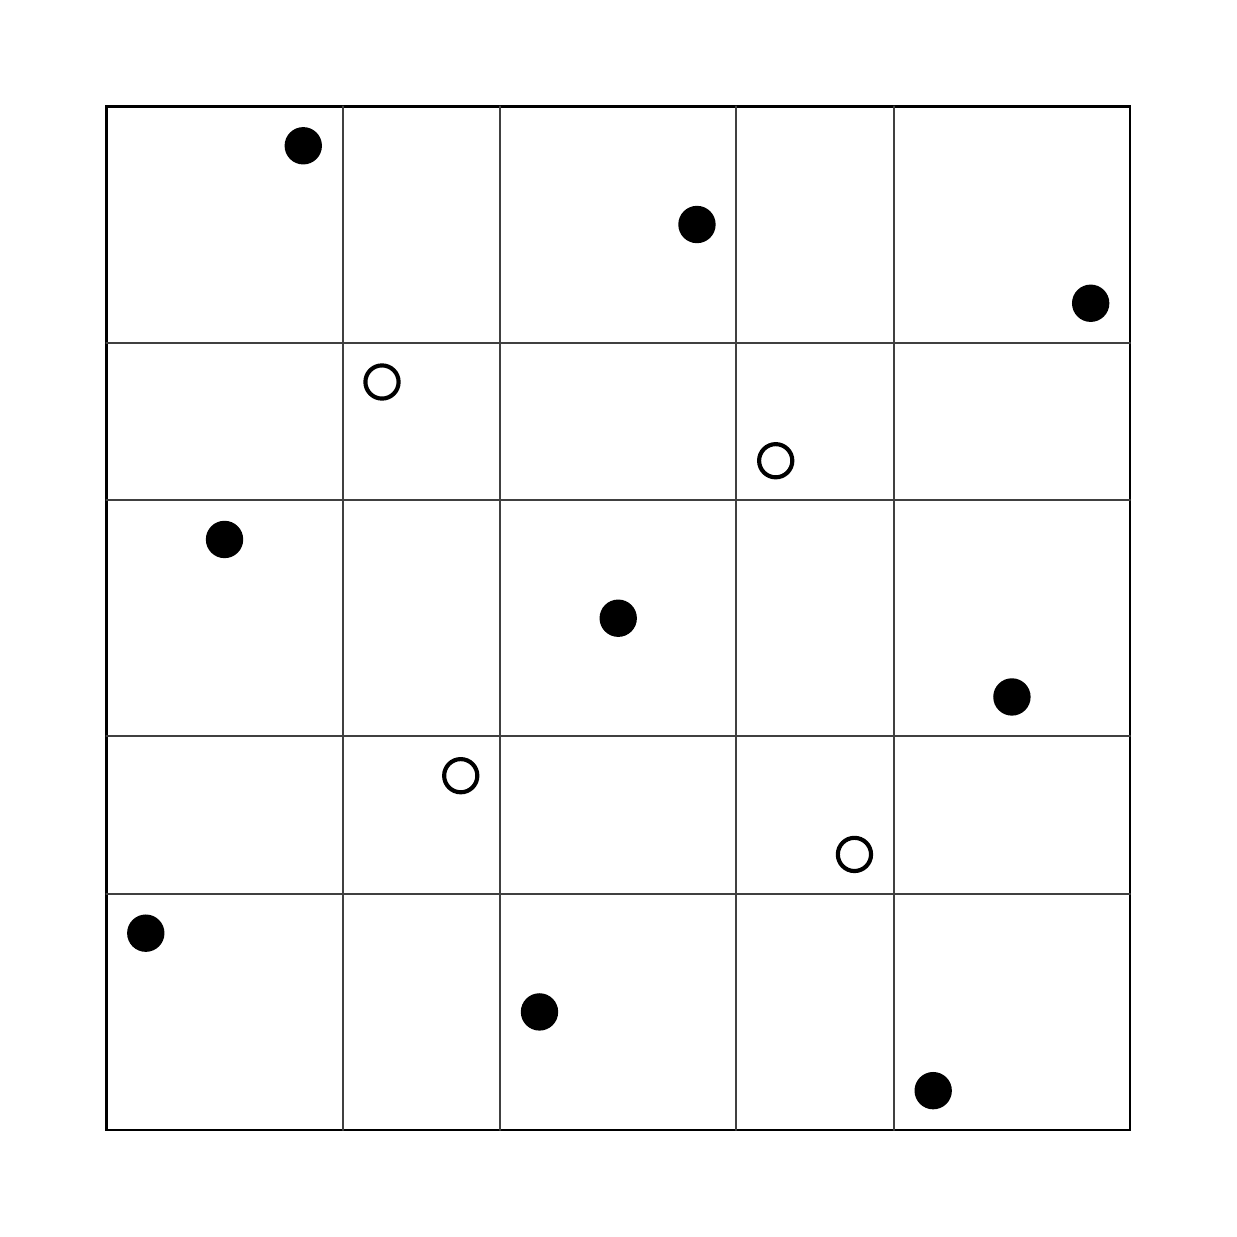
\begin{tikzpicture}[lines]
	\def\size{13}
	
	% Background, frame
	\draw[draw=none, fill=white] (-0.5,-0.5) rectangle ++({\size+2},{\size+2});
	\draw[thick] (0.5,0.5) rectangle ++(\size,\size);

	% Lines
	\begin{scope}[shift={(0.5,0.5)}]
		\foreach \y in {3,5,8,10} {
			\draw[darkgray, thick, line cap=round] (0, \y) -- ++(\size, 0);
			\draw[darkgray, thick, line cap=round] (\y, 0) -- ++(0, \size);
		}
	\end{scope}

	% Points
	\foreach \x/\y in {1/3,2/8,3/13,6/2,7/7,8/12,11/1,12/6,13/11} {
		\draw [fill=black] (\x,\y) circle (6pt);
	}
	\foreach \x/\y in {4/10,5/5,9/9,10/4} {
		\draw (\x,\y) circle (6pt);
	}
	
\end{tikzpicture}
\end{document}